\documentclass[11pt,compress,t,notes=noshow, xcolor=table]{beamer}

\documentclass[11pt,compress,t,notes=noshow, xcolor=table]{beamer}
\usepackage[]{graphicx}\usepackage[]{color}
% maxwidth is the original width if it is less than linewidth
% otherwise use linewidth (to make sure the graphics do not exceed the margin)
\makeatletter
\def\maxwidth{ %
  \ifdim\Gin@nat@width>\linewidth
    \linewidth
  \else
    \Gin@nat@width
  \fi
}
\makeatother

\definecolor{fgcolor}{rgb}{0.345, 0.345, 0.345}
\newcommand{\hlnum}[1]{\textcolor[rgb]{0.686,0.059,0.569}{#1}}%
\newcommand{\hlstr}[1]{\textcolor[rgb]{0.192,0.494,0.8}{#1}}%
\newcommand{\hlcom}[1]{\textcolor[rgb]{0.678,0.584,0.686}{\textit{#1}}}%
\newcommand{\hlopt}[1]{\textcolor[rgb]{0,0,0}{#1}}%
\newcommand{\hlstd}[1]{\textcolor[rgb]{0.345,0.345,0.345}{#1}}%
\newcommand{\hlkwa}[1]{\textcolor[rgb]{0.161,0.373,0.58}{\textbf{#1}}}%
\newcommand{\hlkwb}[1]{\textcolor[rgb]{0.69,0.353,0.396}{#1}}%
\newcommand{\hlkwc}[1]{\textcolor[rgb]{0.333,0.667,0.333}{#1}}%
\newcommand{\hlkwd}[1]{\textcolor[rgb]{0.737,0.353,0.396}{\textbf{#1}}}%
\let\hlipl\hlkwb

\usepackage{framed}
\makeatletter
\newenvironment{kframe}{%
 \def\at@end@of@kframe{}%
 \ifinner\ifhmode%
  \def\at@end@of@kframe{\end{minipage}}%
  \begin{minipage}{\columnwidth}%
 \fi\fi%
 \def\FrameCommand##1{\hskip\@totalleftmargin \hskip-\fboxsep
 \colorbox{shadecolor}{##1}\hskip-\fboxsep
     % There is no \\@totalrightmargin, so:
     \hskip-\linewidth \hskip-\@totalleftmargin \hskip\columnwidth}%
 \MakeFramed {\advance\hsize-\width
   \@totalleftmargin\z@ \linewidth\hsize
   \@setminipage}}%
 {\par\unskip\endMakeFramed%
 \at@end@of@kframe}
\makeatother

\definecolor{shadecolor}{rgb}{.97, .97, .97}
\definecolor{messagecolor}{rgb}{0, 0, 0}
\definecolor{warningcolor}{rgb}{1, 0, 1}
\definecolor{errorcolor}{rgb}{1, 0, 0}
\newenvironment{knitrout}{}{} % an empty environment to be redefined in TeX

\usepackage{alltt}
\newcommand{\SweaveOpts}[1]{}  % do not interfere with LaTeX
\newcommand{\SweaveInput}[1]{} % because they are not real TeX commands
\newcommand{\Sexpr}[1]{}       % will only be parsed by R
\newcommand{\xmark}{\ding{55}}%


\usepackage[english]{babel}
\usepackage[utf8]{inputenc}

\usepackage{dsfont}
\usepackage{verbatim}
\usepackage{amsmath}
\usepackage{amsfonts}
\usepackage{amssymb}
\usepackage{bm}
\usepackage{csquotes}
\usepackage{multirow}
\usepackage{longtable}
\usepackage{booktabs}
\usepackage{enumerate}
\usepackage[absolute,overlay]{textpos}
\usepackage{psfrag}
\usepackage{algorithm}
\usepackage{algpseudocode}
\usepackage{eqnarray}
\usepackage{arydshln}
\usepackage{tabularx}
\usepackage{placeins}
\usepackage{tikz}
\usepackage{setspace}
\usepackage{colortbl}
\usepackage{mathtools}
\usepackage{wrapfig}
\usepackage{bm}
\usepackage{amsmath}
\usepackage{pifont}

\usetikzlibrary{shapes,arrows,automata,positioning,calc,chains,trees, shadows}
\tikzset{
  %Define standard arrow tip
  >=stealth',
  %Define style for boxes
  punkt/.style={
    rectangle,
    rounded corners,
    draw=black, very thick,
    text width=6.5em,
    minimum height=2em,
    text centered},
  % Define arrow style
  pil/.style={
    ->,
    thick,
    shorten <=2pt,
    shorten >=2pt,}
}

\usepackage{subfig}

% Defines macros and environments
\usepackage{../../style/lmu-lecture}


\let\code=\texttt
\let\proglang=\textsf

\setkeys{Gin}{width=0.9\textwidth}

\setbeamertemplate{frametitle}{\expandafter\uppercase\expandafter\insertframetitle}

\usepackage{bbm}
% basic latex stuff
\newcommand{\pkg}[1]{{\fontseries{b}\selectfont #1}} %fontstyle for R packages
\newcommand{\lz}{\vspace{0.5cm}} %vertical space
\newcommand{\dlz}{\vspace{1cm}} %double vertical space
\newcommand{\oneliner}[1] % Oneliner for important statements
{\begin{block}{}\begin{center}\begin{Large}#1\end{Large}\end{center}\end{block}}


%new environments
\newenvironment{vbframe}  %frame with breaks and verbatim
{
 \begin{frame}[containsverbatim,allowframebreaks]
}
{
\end{frame}
}

\newenvironment{vframe}  %frame with verbatim without breaks (to avoid numbering one slided frames)
{
 \begin{frame}[containsverbatim]
}
{
\end{frame}
}

\newenvironment{blocki}[1]   % itemize block
{
 \begin{block}{#1}\begin{itemize}
}
{
\end{itemize}\end{block}
}

\newenvironment{fragileframe}[2]{  %fragile frame with framebreaks
\begin{frame}[allowframebreaks, fragile, environment = fragileframe]
\frametitle{#1}
#2}
{\end{frame}}


\newcommand{\myframe}[2]{  %short for frame with framebreaks
\begin{frame}[allowframebreaks]
\frametitle{#1}
#2
\end{frame}}

\newcommand{\remark}[1]{
  \textbf{Remark:} #1
}


\newenvironment{deleteframe}
{
\begingroup
\usebackgroundtemplate{
\includegraphics[width=\paperwidth,height=\paperheight]{../style/color/red.png}}
 \begin{frame}
}
{
\end{frame}
\endgroup
}
\newenvironment{simplifyframe}
{
\begingroup
\usebackgroundtemplate{
\includegraphics[width=\paperwidth,height=\paperheight]{../style/color/yellow.png}}
 \begin{frame}
}
{
\end{frame}
\endgroup
}\newenvironment{draftframe}
{
\begingroup
\usebackgroundtemplate{
\includegraphics[width=\paperwidth,height=\paperheight]{../style/color/green.jpg}}
 \begin{frame}
}
{
\end{frame}
\endgroup
}
% https://tex.stackexchange.com/a/261480: textcolor that works in mathmode
\makeatletter
\renewcommand*{\@textcolor}[3]{%
  \protect\leavevmode
  \begingroup
    \color#1{#2}#3%
  \endgroup
}
\makeatother





% math spaces
\ifdefined\N                                                                
\renewcommand{\N}{\mathds{N}} % N, naturals
\else \newcommand{\N}{\mathds{N}} \fi 
\newcommand{\Z}{\mathds{Z}} % Z, integers
\newcommand{\Q}{\mathds{Q}} % Q, rationals
\newcommand{\R}{\mathds{R}} % R, reals
\ifdefined\C 
  \renewcommand{\C}{\mathds{C}} % C, complex
\else \newcommand{\C}{\mathds{C}} \fi
\newcommand{\continuous}{\mathcal{C}} % C, space of continuous functions
\newcommand{\M}{\mathcal{M}} % machine numbers
\newcommand{\epsm}{\epsilon_m} % maximum error

% counting / finite sets
\newcommand{\setzo}{\{0, 1\}} % set 0, 1
\newcommand{\setmp}{\{-1, +1\}} % set -1, 1
\newcommand{\unitint}{[0, 1]} % unit interval

% basic math stuff
\newcommand{\xt}{\tilde x} % x tilde
\newcommand{\argmax}{\operatorname{arg\,max}} % argmax
\newcommand{\argmin}{\operatorname{arg\,min}} % argmin
\newcommand{\argminlim}{\mathop{\mathrm{arg\,min}}\limits} % argmax with limits
\newcommand{\argmaxlim}{\mathop{\mathrm{arg\,max}}\limits} % argmin with limits  
\newcommand{\sign}{\operatorname{sign}} % sign, signum
\newcommand{\I}{\mathbb{I}} % I, indicator
\newcommand{\order}{\mathcal{O}} % O, order
\newcommand{\pd}[2]{\frac{\partial{#1}}{\partial #2}} % partial derivative
\newcommand{\floorlr}[1]{\left\lfloor #1 \right\rfloor} % floor
\newcommand{\ceillr}[1]{\left\lceil #1 \right\rceil} % ceiling

% sums and products
\newcommand{\sumin}{\sum\limits_{i=1}^n} % summation from i=1 to n
\newcommand{\sumim}{\sum\limits_{i=1}^m} % summation from i=1 to m
\newcommand{\sumjn}{\sum\limits_{j=1}^n} % summation from j=1 to p
\newcommand{\sumjp}{\sum\limits_{j=1}^p} % summation from j=1 to p
\newcommand{\sumik}{\sum\limits_{i=1}^k} % summation from i=1 to k
\newcommand{\sumkg}{\sum\limits_{k=1}^g} % summation from k=1 to g
\newcommand{\sumjg}{\sum\limits_{j=1}^g} % summation from j=1 to g
\newcommand{\meanin}{\frac{1}{n} \sum\limits_{i=1}^n} % mean from i=1 to n
\newcommand{\meanim}{\frac{1}{m} \sum\limits_{i=1}^m} % mean from i=1 to n
\newcommand{\meankg}{\frac{1}{g} \sum\limits_{k=1}^g} % mean from k=1 to g
\newcommand{\prodin}{\prod\limits_{i=1}^n} % product from i=1 to n
\newcommand{\prodkg}{\prod\limits_{k=1}^g} % product from k=1 to g
\newcommand{\prodjp}{\prod\limits_{j=1}^p} % product from j=1 to p

% linear algebra
\newcommand{\one}{\boldsymbol{1}} % 1, unitvector
\newcommand{\zero}{\mathbf{0}} % 0-vector
\newcommand{\id}{\boldsymbol{I}} % I, identity
\newcommand{\diag}{\operatorname{diag}} % diag, diagonal
\newcommand{\trace}{\operatorname{tr}} % tr, trace
\newcommand{\spn}{\operatorname{span}} % span
\newcommand{\scp}[2]{\left\langle #1, #2 \right\rangle} % <.,.>, scalarproduct
\newcommand{\mat}[1]{\begin{pmatrix} #1 \end{pmatrix}} % short pmatrix command
\newcommand{\Amat}{\mathbf{A}} % matrix A
\newcommand{\Deltab}{\mathbf{\Delta}} % error term for vectors

% basic probability + stats
\renewcommand{\P}{\mathds{P}} % P, probability
\newcommand{\E}{\mathds{E}} % E, expectation
\newcommand{\var}{\mathsf{Var}} % Var, variance
\newcommand{\cov}{\mathsf{Cov}} % Cov, covariance
\newcommand{\corr}{\mathsf{Corr}} % Corr, correlation
\newcommand{\normal}{\mathcal{N}} % N of the normal distribution
\newcommand{\iid}{\overset{i.i.d}{\sim}} % dist with i.i.d superscript
\newcommand{\distas}[1]{\overset{#1}{\sim}} % ... is distributed as ...

% machine learning
\newcommand{\Xspace}{\mathcal{X}} % X, input space
\newcommand{\Yspace}{\mathcal{Y}} % Y, output space
\newcommand{\nset}{\{1, \ldots, n\}} % set from 1 to n
\newcommand{\pset}{\{1, \ldots, p\}} % set from 1 to p
\newcommand{\gset}{\{1, \ldots, g\}} % set from 1 to g
\newcommand{\Pxy}{\mathbb{P}_{xy}} % P_xy
\newcommand{\Exy}{\mathbb{E}_{xy}} % E_xy: Expectation over random variables xy
\newcommand{\xv}{\mathbf{x}} % vector x (bold)
\newcommand{\xtil}{\tilde{\mathbf{x}}} % vector x-tilde (bold)
\newcommand{\yv}{\mathbf{y}} % vector y (bold)
\newcommand{\xy}{(\xv, y)} % observation (x, y)
\newcommand{\xvec}{\left(x_1, \ldots, x_p\right)^\top} % (x1, ..., xp) 
\newcommand{\Xmat}{\mathbf{X}} % Design matrix
\newcommand{\allDatasets}{\mathds{D}} % The set of all datasets
\newcommand{\allDatasetsn}{\mathds{D}_n}  % The set of all datasets of size n 
\newcommand{\D}{\mathcal{D}} % D, data
\newcommand{\Dn}{\D_n} % D_n, data of size n
\newcommand{\Dtrain}{\mathcal{D}_{\text{train}}} % D_train, training set
\newcommand{\Dtest}{\mathcal{D}_{\text{test}}} % D_test, test set
\newcommand{\xyi}[1][i]{\left(\xv^{(#1)}, y^{(#1)}\right)} % (x^i, y^i), i-th observation
\newcommand{\Dset}{\left( \xyi[1], \ldots, \xyi[n]\right)} % {(x1,y1)), ..., (xn,yn)}, data
\newcommand{\defAllDatasetsn}{(\Xspace \times \Yspace)^n} % Def. of the set of all datasets of size n 
\newcommand{\defAllDatasets}{\bigcup_{n \in \N}(\Xspace \times \Yspace)^n} % Def. of the set of all datasets 
\newcommand{\xdat}{\left\{ \xv^{(1)}, \ldots, \xv^{(n)}\right\}} % {x1, ..., xn}, input data
\newcommand{\ydat}{\left\{ \yv^{(1)}, \ldots, \yv^{(n)}\right\}} % {y1, ..., yn}, input data
\newcommand{\yvec}{\left(y^{(1)}, \hdots, y^{(n)}\right)^\top} % (y1, ..., yn), vector of outcomes
\renewcommand{\xi}[1][i]{\xv^{(#1)}} % x^i, i-th observed value of x
\newcommand{\yi}[1][i]{y^{(#1)}} % y^i, i-th observed value of y 
\newcommand{\xivec}{\left(x^{(i)}_1, \ldots, x^{(i)}_p\right)^\top} % (x1^i, ..., xp^i), i-th observation vector
\newcommand{\xj}{\xv_j} % x_j, j-th feature
\newcommand{\xjvec}{\left(x^{(1)}_j, \ldots, x^{(n)}_j\right)^\top} % (x^1_j, ..., x^n_j), j-th feature vector
\newcommand{\phiv}{\mathbf{\phi}} % Basis transformation function phi
\newcommand{\phixi}{\mathbf{\phi}^{(i)}} % Basis transformation of xi: phi^i := phi(xi)

%%%%%% ml - models general
\newcommand{\lamv}{\bm{\lambda}} % lambda vector, hyperconfiguration vector
\newcommand{\Lam}{\bm{\Lambda}}	 % Lambda, space of all hpos
% Inducer / Inducing algorithm
\newcommand{\preimageInducer}{\left(\defAllDatasets\right)\times\Lam} % Set of all datasets times the hyperparameter space
\newcommand{\preimageInducerShort}{\allDatasets\times\Lam} % Set of all datasets times the hyperparameter space
% Inducer / Inducing algorithm
\newcommand{\ind}{\mathcal{I}} % Inducer, inducing algorithm, learning algorithm 

% continuous prediction function f
\newcommand{\ftrue}{f_{\text{true}}}  % True underlying function (if a statistical model is assumed)
\newcommand{\ftruex}{\ftrue(\xv)} % True underlying function (if a statistical model is assumed)
\newcommand{\fx}{f(\xv)} % f(x), continuous prediction function
\newcommand{\fdomains}{f: \Xspace \rightarrow \R^g} % f with domain and co-domain
\newcommand{\Hspace}{\mathcal{H}} % hypothesis space where f is from
\newcommand{\fbayes}{f^{\ast}} % Bayes-optimal model
\newcommand{\fxbayes}{f^{\ast}(\xv)} % Bayes-optimal model
\newcommand{\fkx}[1][k]{f_{#1}(\xv)} % f_j(x), discriminant component function
\newcommand{\fh}{\hat{f}} % f hat, estimated prediction function
\newcommand{\fxh}{\fh(\xv)} % fhat(x)
\newcommand{\fxt}{f(\xv ~|~ \thetab)} % f(x | theta)
\newcommand{\fxi}{f\left(\xv^{(i)}\right)} % f(x^(i))
\newcommand{\fxih}{\hat{f}\left(\xv^{(i)}\right)} % f(x^(i))
\newcommand{\fxit}{f\left(\xv^{(i)} ~|~ \thetab\right)} % f(x^(i) | theta)
\newcommand{\fhD}{\fh_{\D}} % fhat_D, estimate of f based on D
\newcommand{\fhDtrain}{\fh_{\Dtrain}} % fhat_Dtrain, estimate of f based on D
\newcommand{\fhDnlam}{\fh_{\Dn, \lamv}} %model learned on Dn with hp lambda
\newcommand{\fhDlam}{\fh_{\D, \lamv}} %model learned on D with hp lambda
\newcommand{\fhDnlams}{\fh_{\Dn, \lamv^\ast}} %model learned on Dn with optimal hp lambda 
\newcommand{\fhDlams}{\fh_{\D, \lamv^\ast}} %model learned on D with optimal hp lambda 

% discrete prediction function h
\newcommand{\hx}{h(\xv)} % h(x), discrete prediction function
\newcommand{\hh}{\hat{h}} % h hat
\newcommand{\hxh}{\hat{h}(\xv)} % hhat(x)
\newcommand{\hxt}{h(\xv | \thetab)} % h(x | theta)
\newcommand{\hxi}{h\left(\xi\right)} % h(x^(i))
\newcommand{\hxit}{h\left(\xi ~|~ \thetab\right)} % h(x^(i) | theta)
\newcommand{\hbayes}{h^{\ast}} % Bayes-optimal classification model
\newcommand{\hxbayes}{h^{\ast}(\xv)} % Bayes-optimal classification model

% yhat
\newcommand{\yh}{\hat{y}} % yhat for prediction of target
\newcommand{\yih}{\hat{y}^{(i)}} % yhat^(i) for prediction of ith targiet
\newcommand{\resi}{\yi- \yih}

% theta
\newcommand{\thetah}{\hat{\theta}} % theta hat
\newcommand{\thetab}{\bm{\theta}} % theta vector
\newcommand{\thetabh}{\bm{\hat\theta}} % theta vector hat
\newcommand{\thetat}[1][t]{\thetab^{[#1]}} % theta^[t] in optimization
\newcommand{\thetatn}[1][t]{\thetab^{[#1 +1]}} % theta^[t+1] in optimization
\newcommand{\thetahDnlam}{\thetabh_{\Dn, \lamv}} %theta learned on Dn with hp lambda
\newcommand{\thetahDlam}{\thetabh_{\D, \lamv}} %theta learned on D with hp lambda
\newcommand{\mint}{\min_{\thetab \in \Theta}} % min problem theta
\newcommand{\argmint}{\argmin_{\thetab \in \Theta}} % argmin theta

% densities + probabilities
% pdf of x 
\newcommand{\pdf}{p} % p
\newcommand{\pdfx}{p(\xv)} % p(x)
\newcommand{\pixt}{\pi(\xv~|~ \thetab)} % pi(x|theta), pdf of x given theta
\newcommand{\pixit}[1][i]{\pi\left(\xi[#1] ~|~ \thetab\right)} % pi(x^i|theta), pdf of x given theta
\newcommand{\pixii}[1][i]{\pi\left(\xi[#1]\right)} % pi(x^i), pdf of i-th x 

% pdf of (x, y)
\newcommand{\pdfxy}{p(\xv,y)} % p(x, y)
\newcommand{\pdfxyt}{p(\xv, y ~|~ \thetab)} % p(x, y | theta)
\newcommand{\pdfxyit}{p\left(\xi, \yi ~|~ \thetab\right)} % p(x^(i), y^(i) | theta)

% pdf of x given y
\newcommand{\pdfxyk}[1][k]{p(\xv | y= #1)} % p(x | y = k)
\newcommand{\lpdfxyk}[1][k]{\log p(\xv | y= #1)} % log p(x | y = k)
\newcommand{\pdfxiyk}[1][k]{p\left(\xi | y= #1 \right)} % p(x^i | y = k)

% prior probabilities
\newcommand{\pik}[1][k]{\pi_{#1}} % pi_k, prior
\newcommand{\lpik}[1][k]{\log \pi_{#1}} % log pi_k, log of the prior
\newcommand{\pit}{\pi(\thetab)} % Prior probability of parameter theta

% posterior probabilities
\newcommand{\post}{\P(y = 1 ~|~ \xv)} % P(y = 1 | x), post. prob for y=1
\newcommand{\postk}[1][k]{\P(y = #1 ~|~ \xv)} % P(y = k | y), post. prob for y=k
\newcommand{\pidomains}{\pi: \Xspace \rightarrow \unitint} % pi with domain and co-domain
\newcommand{\pibayes}{\pi^{\ast}} % Bayes-optimal classification model
\newcommand{\pixbayes}{\pi^{\ast}(\xv)} % Bayes-optimal classification model
\newcommand{\pix}{\pi(\xv)} % pi(x), P(y = 1 | x)
\newcommand{\piv}{\bm{\pi}} % pi, bold, as vector
\newcommand{\pikx}[1][k]{\pi_{#1}(\xv)} % pi_k(x), P(y = k | x)
\newcommand{\pikxt}[1][k]{\pi_{#1}(\xv ~|~ \thetab)} % pi_k(x | theta), P(y = k | x, theta)
\newcommand{\pixh}{\hat \pi(\xv)} % pi(x) hat, P(y = 1 | x) hat
\newcommand{\pikxh}[1][k]{\hat \pi_{#1}(\xv)} % pi_k(x) hat, P(y = k | x) hat
\newcommand{\pixih}{\hat \pi(\xi)} % pi(x^(i)) with hat
\newcommand{\pikxih}[1][k]{\hat \pi_{#1}(\xi)} % pi_k(x^(i)) with hat
\newcommand{\pdfygxt}{p(y ~|~\xv, \thetab)} % p(y | x, theta)
\newcommand{\pdfyigxit}{p\left(\yi ~|~\xi, \thetab\right)} % p(y^i |x^i, theta)
\newcommand{\lpdfygxt}{\log \pdfygxt } % log p(y | x, theta)
\newcommand{\lpdfyigxit}{\log \pdfyigxit} % log p(y^i |x^i, theta)

% probababilistic
\newcommand{\bayesrulek}[1][k]{\frac{\P(\xv | y= #1) \P(y= #1)}{\P(\xv)}} % Bayes rule
\newcommand{\muk}{\bm{\mu_k}} % mean vector of class-k Gaussian (discr analysis) 

% residual and margin
\newcommand{\eps}{\epsilon} % residual, stochastic
\newcommand{\epsi}{\epsilon^{(i)}} % epsilon^i, residual, stochastic
\newcommand{\epsh}{\hat{\epsilon}} % residual, estimated
\newcommand{\yf}{y \fx} % y f(x), margin
\newcommand{\yfi}{\yi \fxi} % y^i f(x^i), margin
\newcommand{\Sigmah}{\hat \Sigma} % estimated covariance matrix
\newcommand{\Sigmahj}{\hat \Sigma_j} % estimated covariance matrix for the j-th class

% ml - loss, risk, likelihood
\newcommand{\Lyf}{L\left(y, f\right)} % L(y, f), loss function
\newcommand{\Lypi}{L\left(y, \pi\right)} % L(y, pi), loss function
\newcommand{\Lxy}{L\left(y, \fx\right)} % L(y, f(x)), loss function
\newcommand{\Lxyi}{L\left(\yi, \fxi\right)} % loss of observation
\newcommand{\Lxyt}{L\left(y, \fxt\right)} % loss with f parameterized
\newcommand{\Lxyit}{L\left(\yi, \fxit\right)} % loss of observation with f parameterized
\newcommand{\Lxym}{L\left(\yi, f\left(\bm{\tilde{x}}^{(i)} ~|~ \thetab\right)\right)} % loss of observation with f parameterized
\newcommand{\Lpixy}{L\left(y, \pix\right)} % loss in classification
\newcommand{\Lpiv}{L\left(y, \piv\right)} % loss in classification
\newcommand{\Lpixyi}{L\left(\yi, \pixii\right)} % loss of observation in classification
\newcommand{\Lpixyt}{L\left(y, \pixt\right)} % loss with pi parameterized
\newcommand{\Lpixyit}{L\left(\yi, \pixit\right)} % loss of observation with pi parameterized
\newcommand{\Lhxy}{L\left(y, \hx\right)} % L(y, h(x)), loss function on discrete classes
\newcommand{\Lr}{L\left(r\right)} % L(r), loss defined on residual (reg) / margin (classif)
\newcommand{\lone}{|y - \fx|} % L1 loss
\newcommand{\ltwo}{\left(y - \fx\right)^2} % L2 loss
\newcommand{\lbernoullimp}{\ln(1 + \exp(-y \cdot \fx))} % Bernoulli loss for -1, +1 encoding
\newcommand{\lbernoullizo}{- y \cdot \fx + \log(1 + \exp(\fx))} % Bernoulli loss for 0, 1 encoding
\newcommand{\lcrossent}{- y \log \left(\pix\right) - (1 - y) \log \left(1 - \pix\right)} % cross-entropy loss
\newcommand{\lbrier}{\left(\pix - y \right)^2} % Brier score
\newcommand{\risk}{\mathcal{R}} % R, risk
\newcommand{\riskbayes}{\mathcal{R}^\ast}
\newcommand{\riskf}{\risk(f)} % R(f), risk
\newcommand{\riskdef}{\E_{y|\xv}\left(\Lxy \right)} % risk def (expected loss)
\newcommand{\riskt}{\mathcal{R}(\thetab)} % R(theta), risk
\newcommand{\riske}{\mathcal{R}_{\text{emp}}} % R_emp, empirical risk w/o factor 1 / n
\newcommand{\riskeb}{\bar{\mathcal{R}}_{\text{emp}}} % R_emp, empirical risk w/ factor 1 / n
\newcommand{\riskef}{\riske(f)} % R_emp(f)
\newcommand{\risket}{\mathcal{R}_{\text{emp}}(\thetab)} % R_emp(theta)
\newcommand{\riskr}{\mathcal{R}_{\text{reg}}} % R_reg, regularized risk
\newcommand{\riskrt}{\mathcal{R}_{\text{reg}}(\thetab)} % R_reg(theta)
\newcommand{\riskrf}{\riskr(f)} % R_reg(f)
\newcommand{\riskrth}{\hat{\mathcal{R}}_{\text{reg}}(\thetab)} % hat R_reg(theta)
\newcommand{\risketh}{\hat{\mathcal{R}}_{\text{emp}}(\thetab)} % hat R_emp(theta)
\newcommand{\LL}{\mathcal{L}} % L, likelihood
\newcommand{\LLt}{\mathcal{L}(\thetab)} % L(theta), likelihood
\newcommand{\LLtx}{\mathcal{L}(\thetab | \xv)} % L(theta|x), likelihood
\newcommand{\logl}{\ell} % l, log-likelihood
\newcommand{\loglt}{\logl(\thetab)} % l(theta), log-likelihood
\newcommand{\logltx}{\logl(\thetab | \xv)} % l(theta|x), log-likelihood
\newcommand{\errtrain}{\text{err}_{\text{train}}} % training error
\newcommand{\errtest}{\text{err}_{\text{test}}} % test error
\newcommand{\errexp}{\overline{\text{err}_{\text{test}}}} % avg training error

% lm
\newcommand{\thx}{\thetab^\top \xv} % linear model
\newcommand{\olsest}{(\Xmat^\top \Xmat)^{-1} \Xmat^\top \yv} % OLS estimator in LM 



\newcommand{\titlefigure}{figure_man/quadratic_functions_2D_example_2_4.png}
\newcommand{\learninggoals}{
\item Geometry of quadratic forms
\item Spectrum of Hessian}


\title{Optimization in Machine Learning}
%\author{Bernd Bischl, Christoph Molnar, Daniel Schalk, Fabian Scheipl}
\date{}

\begin{document}

\lecturechapter{Mathematical Concepts: \\Quadratic forms II}
\lecture{Optimization in Machine Learning}
\sloppy

% ------------------------------------------------------------------------------

\begin{vbframe}{Properties of quadratic functions}

\vspace{-\baselineskip}

\begin{kframe}
    \textbf{Recall}: Quadratic form $q$
    \begin{itemize}
        \item Univariate: $q(x) = ax^2 + bx + c$
        \item Multivariate: $q(\xv) = \xv^T \Amat \xv + \bm{b}^T \xv + c$
    \end{itemize}
\end{kframe}

\textbf{General observation:} If $q\geq0$ ($q\leq0)$, $q$ is convex (concave)

\lz

\textbf{Univariate function:} Second derivative is $q''(x) = 2a$

\begin{itemize}
    \item $q''(x) \overset{(>)}{\geq} 0$: $q$~(strictly) convex. 
        $q''(x) \overset{(<)}{\leq} 0$: $q$~(strictly) concave.
    \item High (low) absolute values of $q''(x)$: high (low) curvature
\end{itemize}

\lz

\textbf{Multivariate function:} Second derivative is $\mathbf{H}=2\Amat$

\begin{itemize}
    \item Convexity/concavity of~$q$ depend on eigenvalues of~$\mathbf{H}$
    \item Let us look at an example of the form $q(\xv) = \xv^T\Amat\xv$
\end{itemize}

\end{vbframe}
  
\begin{vbframe}{Geometry of quadratic functions}

% \textbf{Example 1}: Function composed of two univariate quadratic terms

% \vspace*{-0.3cm}

% \only<1>{
%     \begin{eqnarray*}
%         q(\xv) &=& \xv^T \Amat \xv = \xv^T\begin{pmatrix} 2 & 0 \\ 0 & 1\end{pmatrix} \xv = 2 \cdot x_1^2 + x_2^2 \\
%         \text{with } \nabla q(\xv) &=& 2 \cdot \Amat \cdot \xv = 4 \cdot x_1 + 2 \cdot x_2, \quad \bm{H} = 2 \cdot \Amat = \begin{pmatrix} \textcolor{orange}{4} & 0 \\ 0 & 2 \end{pmatrix} 
%     \end{eqnarray*}
% }

% \only<2>{
%     \begin{eqnarray*}
%         q(\xv) &=& \xv^T \Amat \xv = \xv^T\begin{pmatrix} 2 & 0 \\ 0 & 1\end{pmatrix} \xv = 2 \cdot x_1^2 + x_2^2 \\
%         \text{with } \nabla q(\xv) &=& 2 \cdot \Amat \cdot \xv = 4 \cdot x_1 + 2 \cdot x_2, \quad \bm{H} = 2 \cdot \Amat = \begin{pmatrix} \textcolor{orange}{4} & 0 \\ 0 & \textcolor{magenta}{2} \end{pmatrix} 
%     \end{eqnarray*}
% }

% \begin{figure}
%     \only<1>{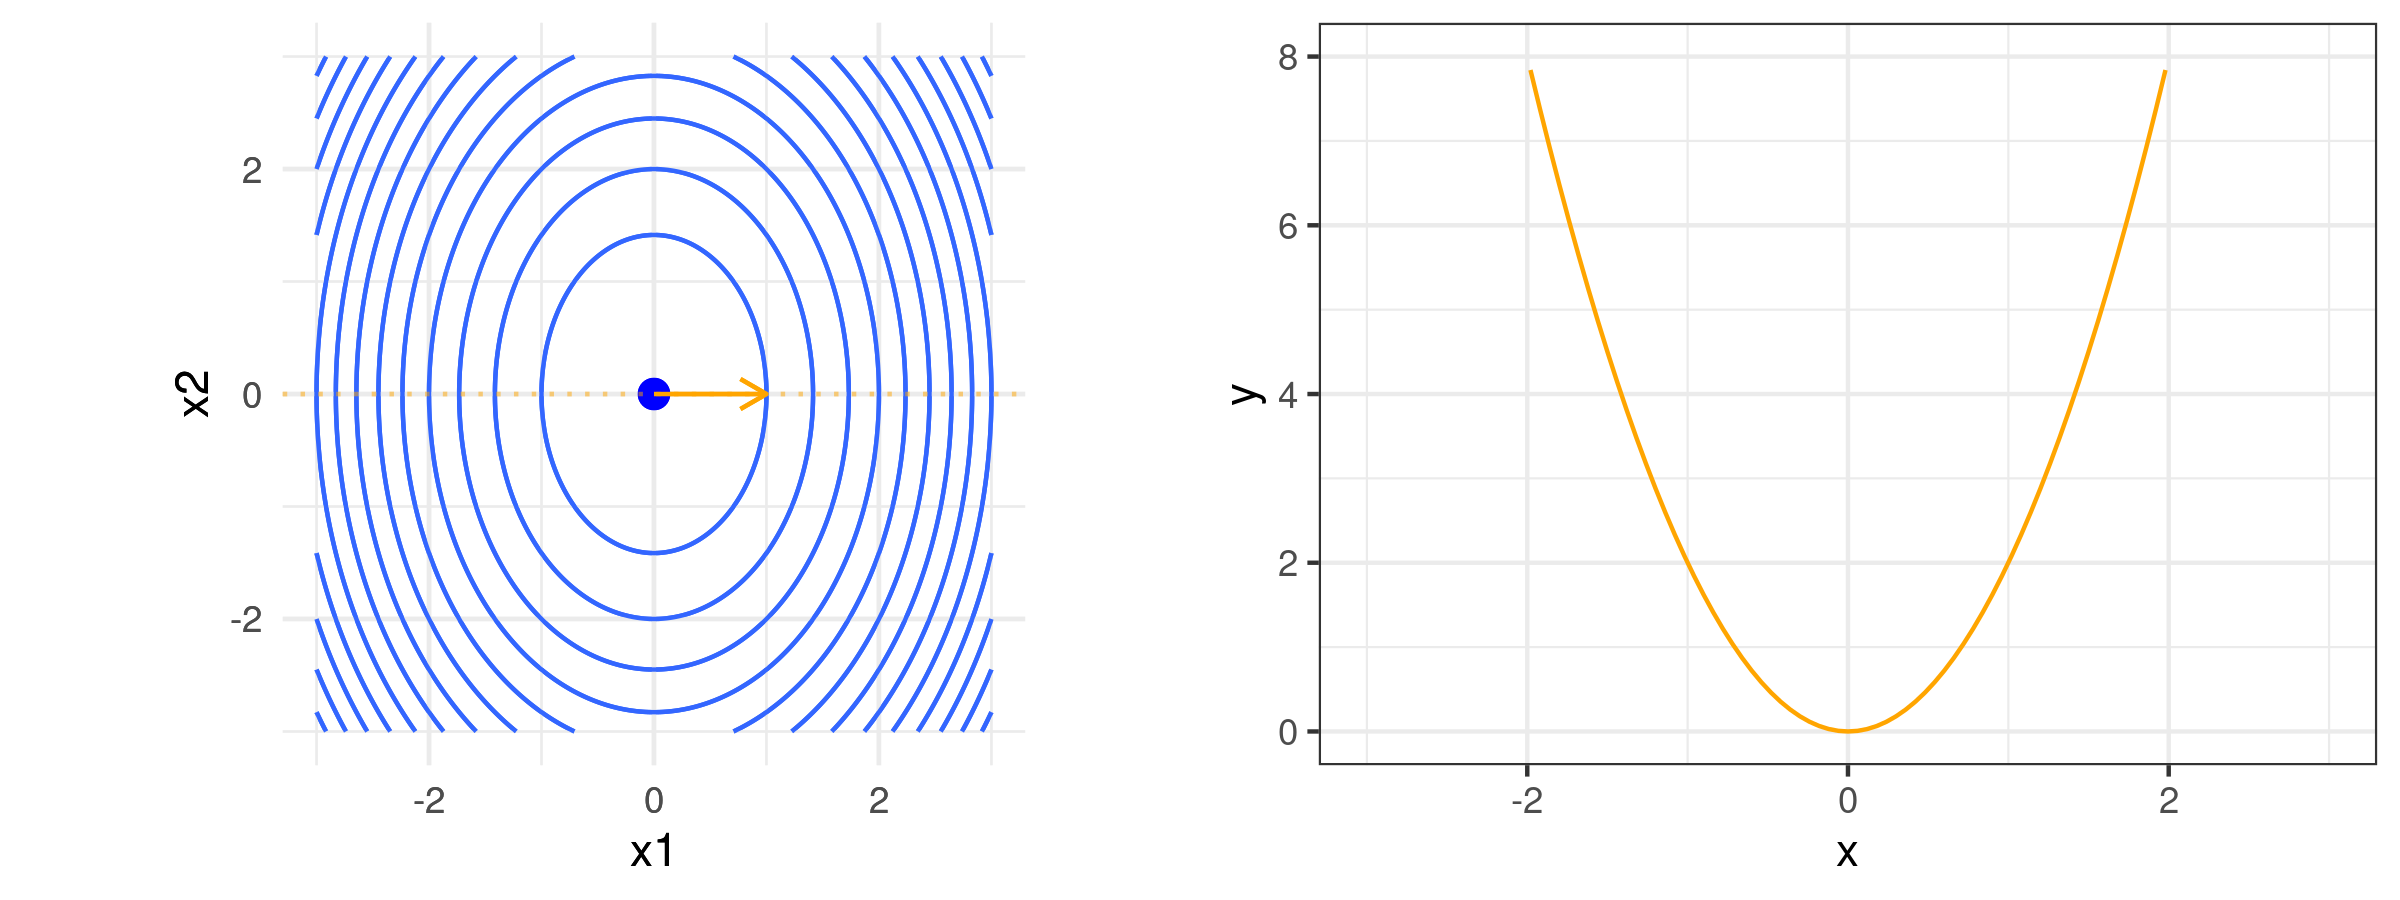
\includegraphics[height=0.4\textwidth, keepaspectratio]{figure_man/quadratic_functions_2D_example_diag_2.png} \\
%         \begin{footnotesize} 
%             $q$ has a high positive curvature of $\textcolor{orange}{4}$ in the direction of $\textcolor{orange}{v = (1, 0)^T}$, \phantom{mand a lower (positive) curvature off $\textcolor{magenta}{2}$ in direction of $\textcolor{magenta}{v = (0, 1)^T}$.}
%         \end{footnotesize}
%     }
%     \only<2>{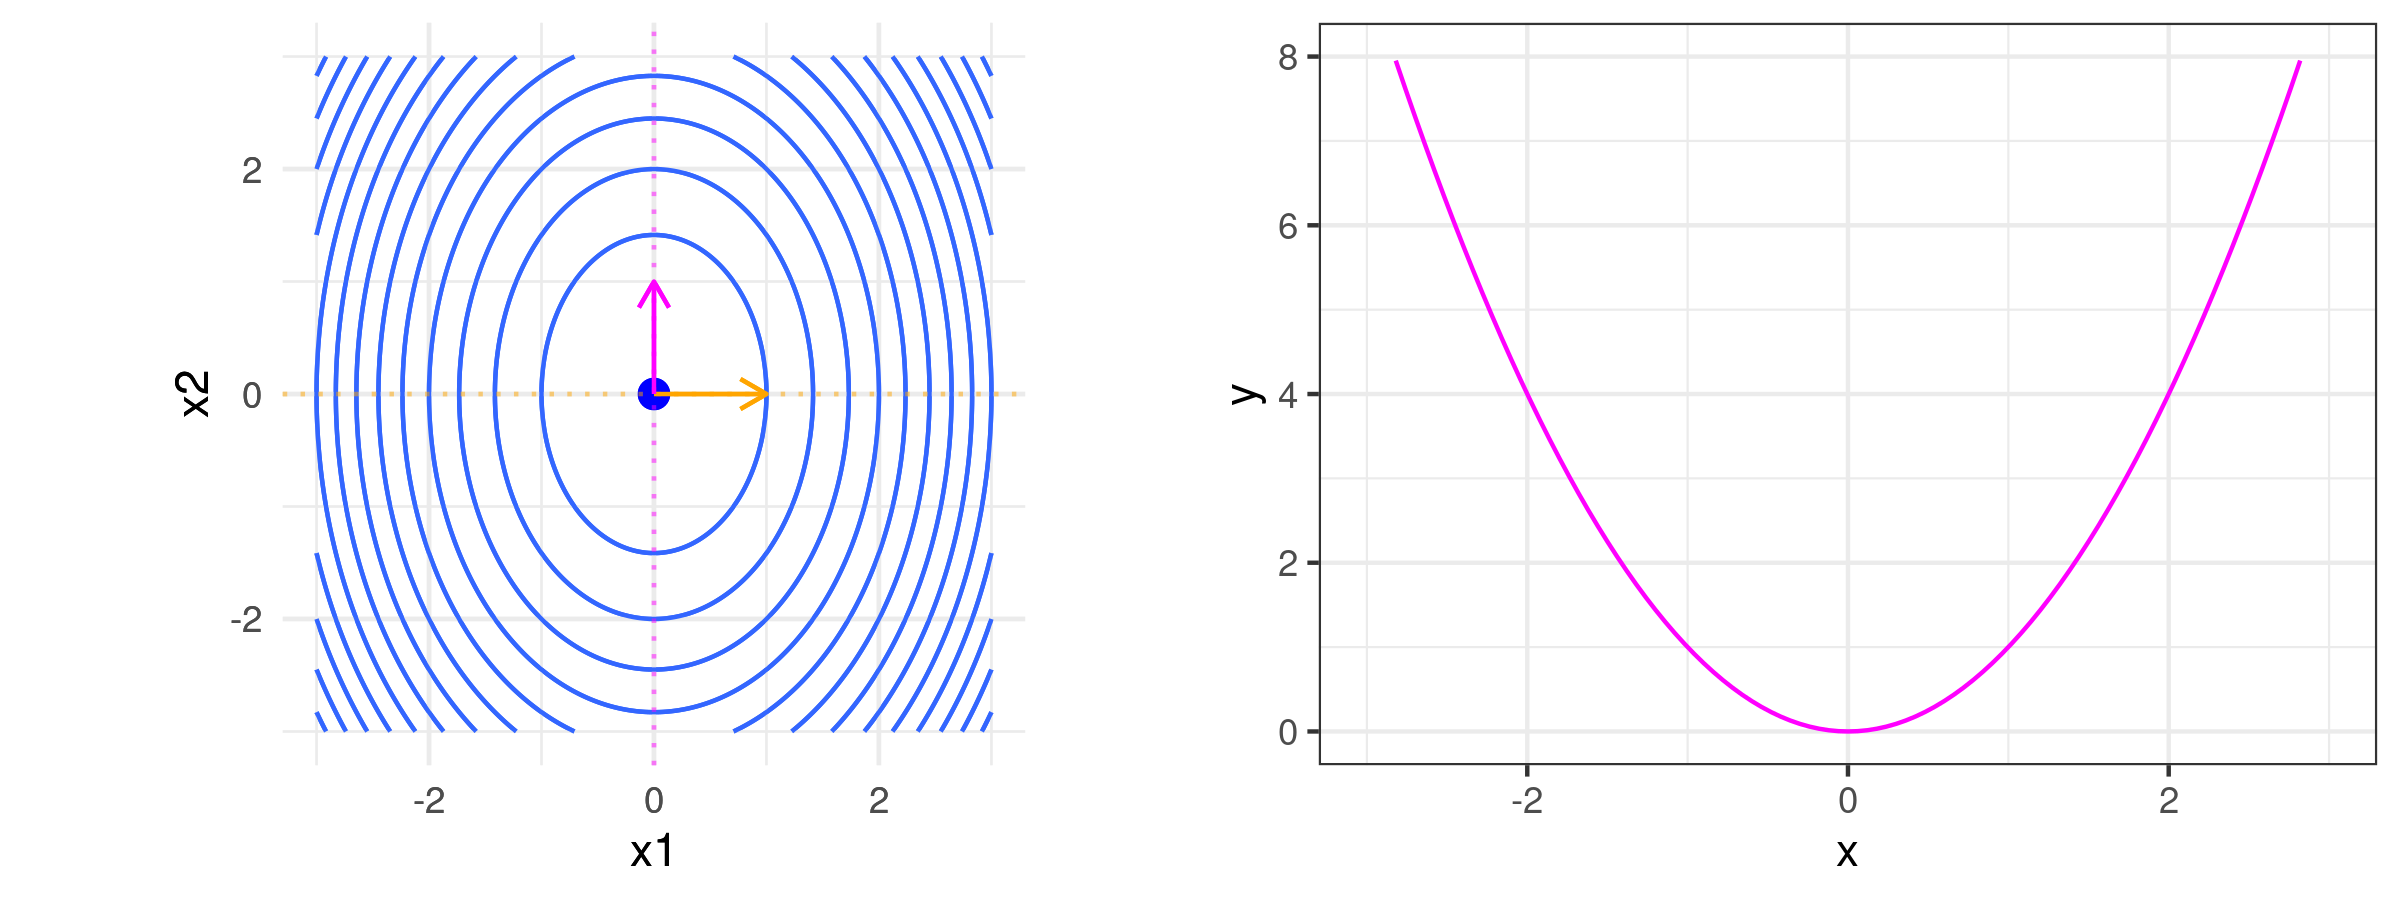
\includegraphics[height=0.4\textwidth, keepaspectratio]{figure_man/quadratic_functions_2D_example_diag_3.png} \\
%         \begin{footnotesize} 
%             $q$ has a high positive curvature of $\textcolor{orange}{4}$ in the direction of $\textcolor{orange}{v = (1, 0)^T}$, and a lower (positive) curvature of $\textcolor{magenta}{2}$ in direction of $\textcolor{magenta}{v = (0, 1)^T}$.
%         \end{footnotesize}
%     }
% \end{figure}

% \framebreak  
  
% \textbf{Takeaway I}: 

% \begin{itemize}
%     \item Hessian encodes curvature 
%     \item If the Hessian $\mathbf{H}$ is diagonal, the diagonal elements encode the curvature of the function: 
    
%         \begin{itemize}
%             \item $i$-th diagonal element gives us the curvature in the direction of $\bm{v} = \bm{e}_i$ because 
%                 $$
%                 \bm{v}^T \bm{H} \bm{v} = \bm{e}_i^T \bm{H} \bm{e}_i = h_{ii}.
%                 $$
%             \item The curvature in an arbitrary direction $\bm{v}
%                 \in \R^d$, $\|\bm{v}\| = 1$, is 
%                 $$
%                 \bm{v}^T\mathbf{H}\bm{v} = h_{11} v_1^2 + h_{22}v_2^2 + ... + h_{dd}v_d^2. 
%                 $$
%         \end{itemize}

%     \item<2-> For general (non-diagonal) matrices we analyze the \textbf{eigenspectrum} of $\mathbf{H}$ 
%     \vspace*{0.2cm}
%     \item<2->[]
%         \begin{footnotesize}
%             \textbf{Note: } For diagonal matrices the eigenspectrum is is to read-off: Diagonal elements of $\mathbf{H}$ \textbf{eigenvalues}, unit vectors \textbf{eigenvectors}
%             \begin{eqnarray*}
%                 \mathbf{H} \bm{e}_1 &=& \begin{pmatrix} \textcolor{orange}{4} & 0 \\ 0 & \textcolor{magenta}{2} \end{pmatrix} = \textcolor{orange}{4} \cdot \bm{e}_1; \qquad \mathbf{H} \bm{e}_2 = \begin{pmatrix} \textcolor{orange}{4} & 0 \\ 0 & \textcolor{magenta}{2} \end{pmatrix} = \textcolor{magenta}{2} \cdot \bm{e}_2 \\		
%             \end{eqnarray*}	
%         \end{footnotesize}
    
% \end{itemize}

% \framebreak
  
\textbf{Example:} $\Amat = \begin{pmatrix} 2 & -1 \\ -1 & 2\end{pmatrix}$ $\implies$ $\mathbf{H} = 2\Amat = \begin{pmatrix} 4 & -2 \\ -2 & 4\end{pmatrix}$

% \only<1>{
% 	\begin{figure}
% 		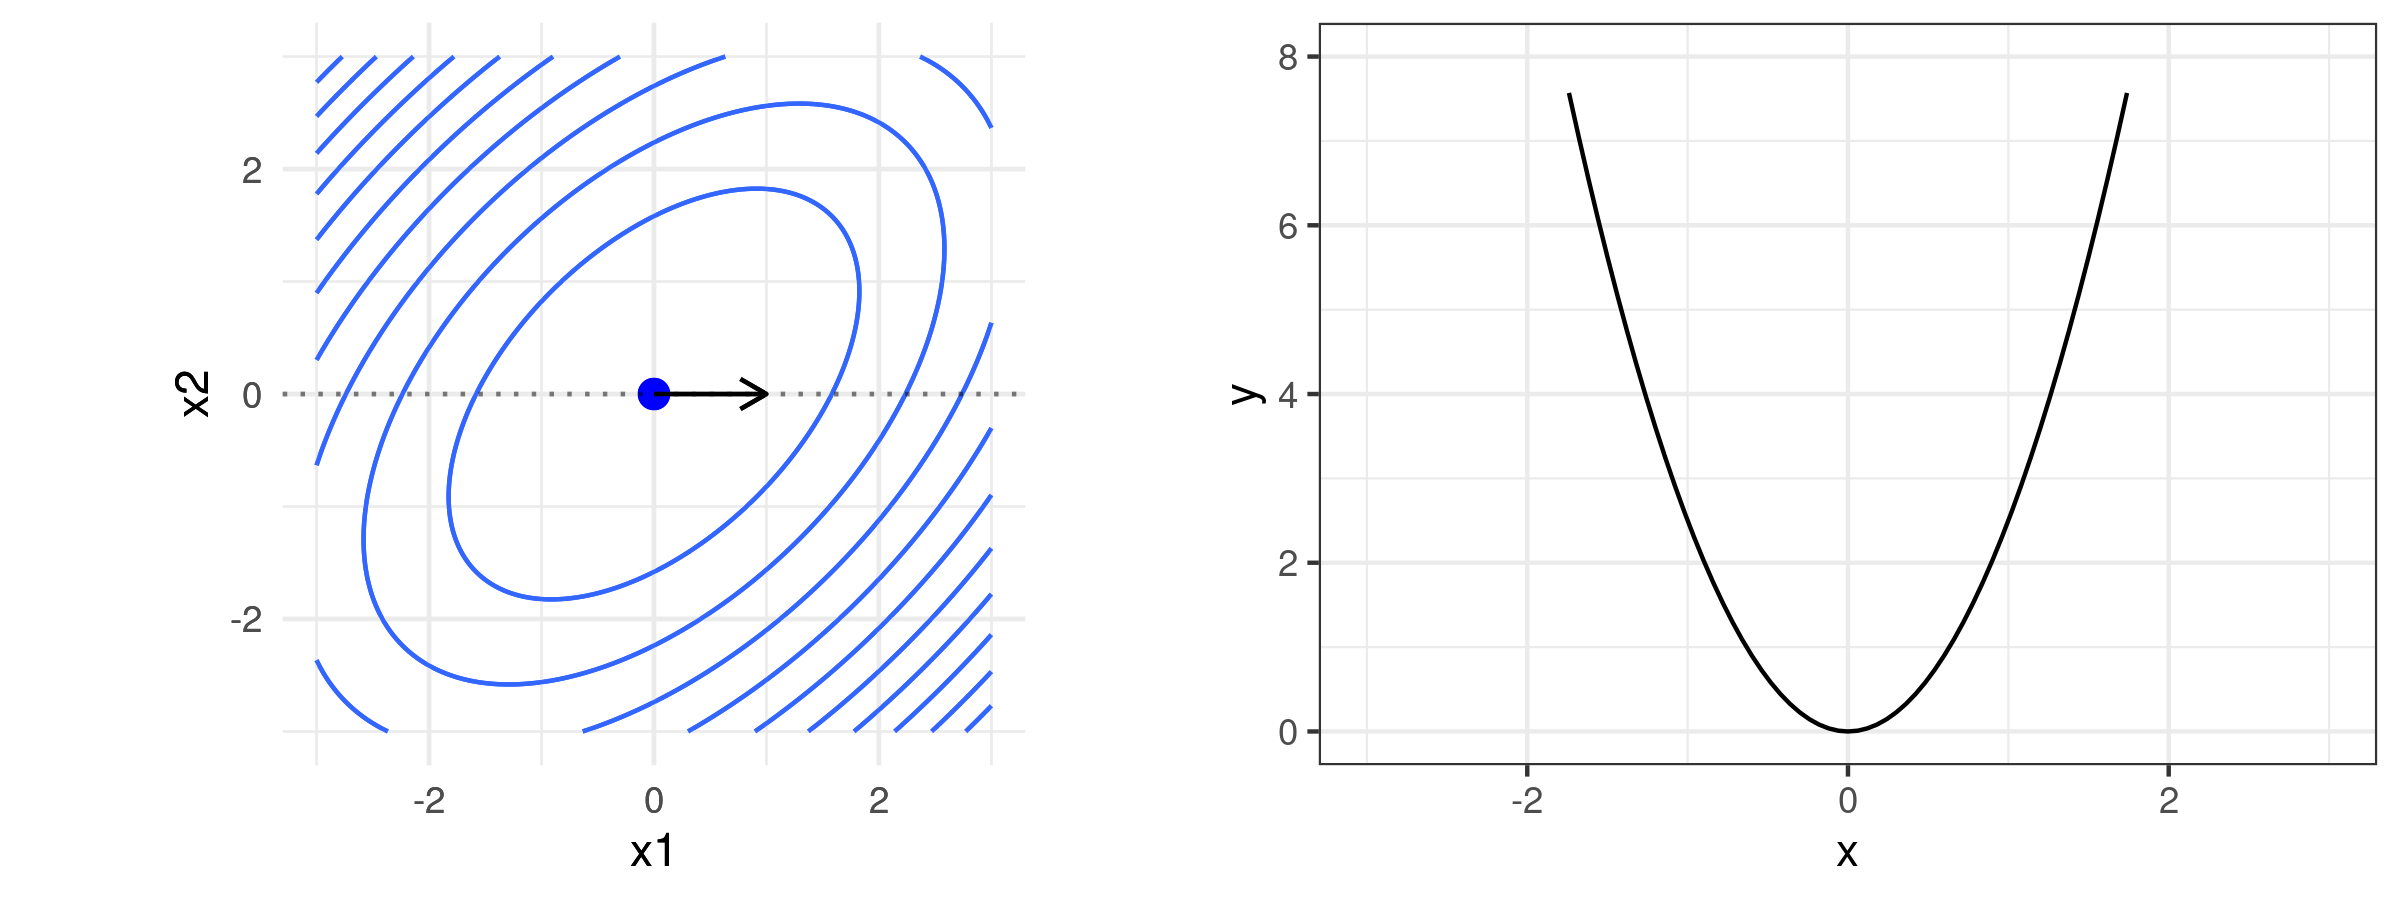
\includegraphics[height=0.4\textwidth, keepaspectratio]{figure_man/quadratic_functions_2D_example_1_3.png} \\
% 		\begin{footnotesize} 
% 			We can again look at the (directional) curvature along the $x_1$ axis, \phantom{ or $x_2$ axis. However, there is a direction of maximum and minimum curvature. } 
% 		\end{footnotesize}
% 	\end{figure}
% }

% \only<2>{
% 	\begin{figure}
% 		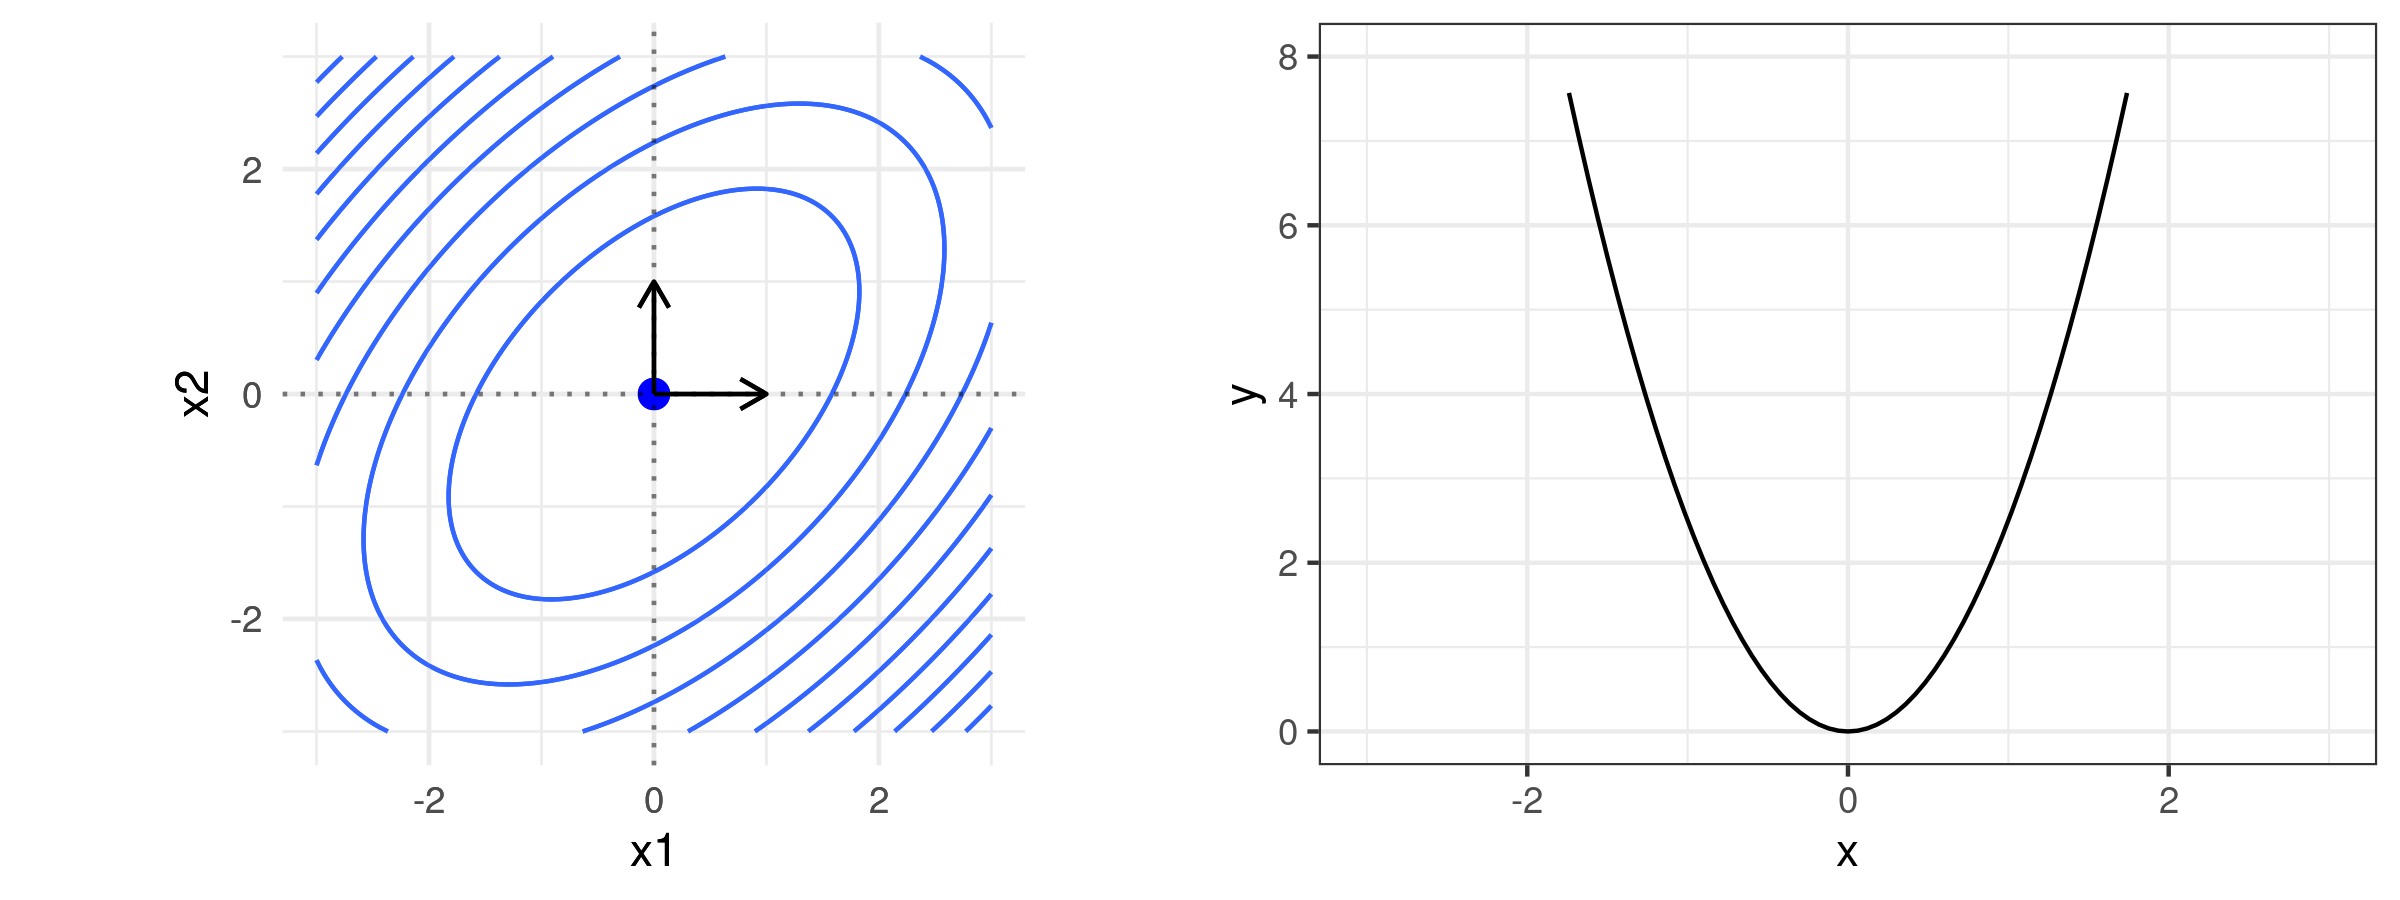
\includegraphics[height=0.4\textwidth, keepaspectratio]{figure_man/quadratic_functions_2D_example_1_4.png} \\
% 		\begin{footnotesize} 
% 			We can again look at the (directional) curvature along the $x_1$ axis, or $x_2$ axis. \phantom{The directions of maximum and minimum curvature are along the eigenvectors of $\bm{H}$. } 
% 		\end{footnotesize}
% 	\end{figure}
% }

\begin{itemize}
    \item Since~$\mathbf{H}$ symmetric, eigendecomposition $\mathbf{H} = \mathbf{V}\Lambda\mathbf{V}^T$ with
        \begin{equation*}
            \mathbf{V} = \begin{pmatrix}
                    | & | \\
                    \textcolor{magenta}{v_\text{max}} & \textcolor{orange}{v_\text{min}} \\
                    | & |
                \end{pmatrix}
                = \frac{1}{\sqrt{2}} \begin{pmatrix}
                    1 & 1 \\
                    -1 & 1
                \end{pmatrix}
            \text{ orthogonal}
        \end{equation*}
        \begin{equation*}
            \text{and }
            \Lambda = \begin{pmatrix}
                \textcolor{magenta}{\lambda_\text{max}} & 0 \\
                0 & \textcolor{orange}{\lambda_\text{min}}
            \end{pmatrix}
            = \begin{pmatrix}6 & 0 \\ 0 & 2\end{pmatrix}.
        \end{equation*}
\end{itemize}

\vspace{-0.5\baselineskip}

\begin{figure}
    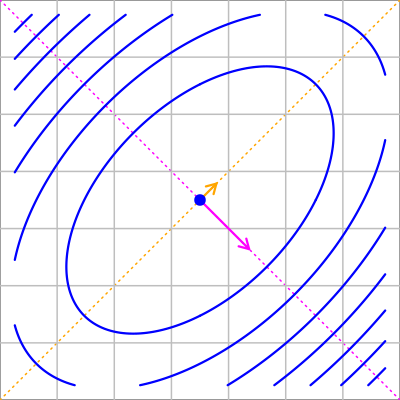
\includegraphics[height=0.28\textwidth,keepaspectratio]{figure_man/quadr-eigenv.png}
\end{figure}
  
\framebreak
    
\begin{itemize}
    \item $\textcolor{magenta}{\bm{v}_\text{max}}$ ($\textcolor{orange}{\bm{v}_\text{min}}$) direction of highest (lowest) curvature

        \vspace{0.25\baselineskip}
    
        \begin{footnotesize}
            \textbf{Proof:} With $\bm{v}=\mathbf{V}^T\xv$:

            \vspace{-\baselineskip}
            
            \begin{equation*}
                \xv^T\Amat\xv = \xv^T\mathbf{V}\Lambda\mathbf{V}^T\xv = \bm{v}^T\Lambda\bm{v} = \sum_{i=1}^d \lambda_iv_i^2 \leq \textcolor{magenta}{\lambda_\text{max}} \sum_{i=1}^d v_i^2 = \textcolor{magenta}{\lambda_\text{max}}\|\bm{v}\|^2
            \end{equation*}
            Since $\|\bm{v}\| = \|\xv\|$ ($\mathbf{V}$ orthogonal): $\max_{\|\xv\|=1} \xv^T\Amat\xv \leq \textcolor{magenta}{\lambda_\text{max}}$
            
            Additional: $\textcolor{magenta}{\bm{v}_\text{max}}^T\Amat\textcolor{magenta}{\bm{v}_\text{max}} = \mathbf{e}_1^T\Lambda\mathbf{e}_1 = \textcolor{magenta}{\lambda_\text{max}}$

            Analogous: $\min_{\|\xv\|=1} \xv^T \Amat \xv \geq \textcolor{orange}{\lambda_\text{min}}$ and $\textcolor{orange}{\bm{v}_\text{min}}^T\Amat\textcolor{orange}{\bm{v}_\text{min}} = \textcolor{orange}{\lambda_\text{min}}$
        \end{footnotesize}

    \medskip

    \item $\textcolor{magenta}{\bm{v}_\text{max}}$,$\textcolor{orange}{\bm{v}_\text{min}}$ principal axes of contour ellipses (principal axis theorem)

        \vspace{0.25\baselineskip}
    
        \begin{footnotesize}
            \textbf{Proof:} With $\bm{v}=\mathbf{V}^T\xv$:

            \vspace{-0.5\baselineskip}

            \begin{equation*}
                q(\xv) = \xv^T\Amat\xv + \bm{b}^T\xv + c = \bm{v}^T\Lambda\bm{v} + \bm{b}^T V \bm{v} + c =: \tilde{q}(\bm{v})
            \end{equation*}

            Now:
            \begin{equation*}
                q(\bm{v}_j) = \mathbf{e}_j^T\Lambda\mathbf{e}_j + \bm{b}^T V \mathbf{e}_j + c = \tilde{q}(\mathbf{e}_j)
            \end{equation*}

            Especially: $q(\textcolor{magenta}{\bm{v}_\text{max}}) = \textcolor{magenta}{\lambda_\text{max}} = \tilde{q}(\mathbf{e}_1) \quad\text{and}\quad q(\textcolor{orange}{\bm{v}_\text{min}}) = \textcolor{orange}{\lambda_\text{min}} = \tilde{q}(\mathbf{e}_d)$
        \end{footnotesize}
\end{itemize}

Recall: \textbf{Second order condition for optimality} is \textbf{sufficient}.

\medskip

We skipped the \textbf{proof} at first, but can now catch up on it.

\begin{kframe}
    \footnotesize
     If $H(\xv^\ast) \succ 0$ at stationary point~$\xv^\ast$, then $\xv^\ast$ is local minimum ($\prec$ for maximum).

     \medskip

    \textbf{Proof:}
    Let $\textcolor{orange}{\lambda_\text{min}}>0$ denote the smallest eigenvalue of $H(\xv^\ast)$.
    Then:
    
    \vspace{-1.25\baselineskip}
    
    \begin{equation*}
        f(\xv) = f(\xv^\ast) + \underbrace{\nabla f(\xv^\ast)}_{=0}{}^T(\xv-\xv^\ast) + \frac{1}{2}\underbrace{(\xv-\xv^\ast)^T H(\xv^\ast)(\xv-\xv^\ast)}_{\geq \textcolor{orange}{\lambda_\text{min}} \|\xv-\xv^\ast\|^2 \text{ (see above)}} + \underbrace{R_2(\xv,\xv^\ast)}_{=o(\|\xv-\xv^\ast\|^2)}.
    \end{equation*}

    Choose~$\eps>0$ s.t. $|R_2(\xv,\xv^\ast)| < \frac{1}{2} \textcolor{orange}{\lambda_\text{min}} \|\xv-\xv^\ast\|^2$ for each~$\xv$ with $\|\xv-\xv^\ast\|<\eps$.
    Then:

    \vspace{-1.25\baselineskip}

    \begin{equation*}
        f(\xv) \geq f(\xv^\ast) + \underbrace{\frac{1}{2} \textcolor{orange}{\lambda_\text{min}} \|\xv-\xv^\ast\|^2 + R_2(\xv,\xv^\ast)}_{>0} > f(\xv^\ast) \quad\text{for each $\xv$ with $\|\xv-\xv^\ast\|<\eps$}.
    \end{equation*}
\end{kframe}

\framebreak

If spectrum of~$\Amat$ is known, also that of $\mathbf{H} = 2\Amat$ is known.

\begin{itemize}
    \item If \textbf{all} eigenvalues of $\mathbf{H}$ $\overset{(>)}{\geq} 0$ ($\Leftrightarrow$ $\mathbf{H} \overset{(\succ)}{\succcurlyeq} 0$):
        \begin{itemize} 
            \item $q$ (strictly) convex,
            \item there is a (unique) global minimum. 
        \end{itemize}
    \item If \textbf{all} eigenvalues of $\mathbf{H}$ $\overset{(<)}{\leq} 0$ ($\Leftrightarrow$ $\mathbf{H} \overset{(\prec)}{\preccurlyeq} 0$):
        \begin{itemize} 
            \item $q$ (strictly) concave,
            \item there is a (unique) global maximum. 
        \end{itemize}
    \item If~$\mathbf{H}$ has both positive and negative eigenvalues ($\Leftrightarrow$ $\mathbf{H}$ indefinite):
        \begin{itemize}
            \item $q$ neither convex nor concave,
            \item there is a saddle point.
        \end{itemize}
\end{itemize}

% \begin{figure}
%     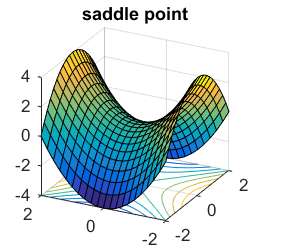
\includegraphics[width=0.3\textwidth, keepaspectratio]{figure_man/minmaxsaddle_2.png}
% \end{figure}

\begin{figure}
    \centering
    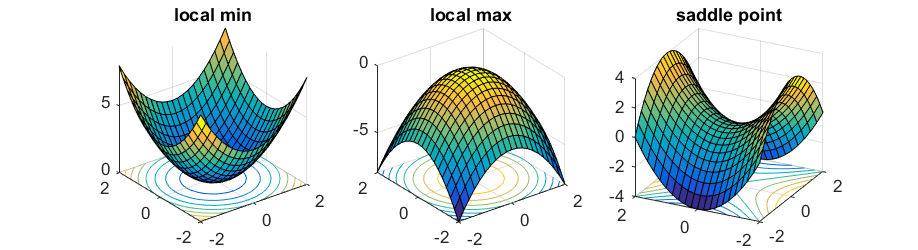
\includegraphics[width=0.67\textwidth]{figure_man/minmaxsaddle.png}
\end{figure}

\end{vbframe}

\begin{vbframe}{Condition and curvature}

Condition of~$\mathbf{H} = 2\Amat$ is given by $\kappa(\mathbf{H}) = \kappa(\Amat) = |\textcolor{magenta}{\lambda_\text{max}}| / |\textcolor{orange}{\lambda_\text{min}}|$.

\vspace{\baselineskip}

\textbf{High condition} means: 

\begin{itemize}
    \item $|\textcolor{magenta}{\lambda_\text{max}}| \gg |\textcolor{orange}{\lambda_\text{min}}|$
    \item Curvature along $\textcolor{magenta}{\bm{v}_\text{max}}$ $\gg$ curvature along $\textcolor{orange}{\bm{v}_\text{min}}$
    \item \textbf{Problem} for optimization algorithms like \textbf{gradient descent} (later)
\end{itemize}

\begin{figure}
    \centering
    
\includegraphics[width=\textwidth]{figure_man/quadr-conds.png}
    \caption*{\footnotesize \textbf{Left:} Excellent condition. \textbf{Middle:} Good condition. \textbf{Right:} Bad condition.}
\end{figure}

\end{vbframe}

\begin{vbframe}{Approximation of smooth functions}

Any function~$f \in \mathcal{C}^2$ can be locally approximated by a quadratic function via second order Taylor approximation: 

\vspace*{-0.5\baselineskip}

\begin{equation*}
    f(\xv) \approx f(\bm{\tilde{x}}) + \nabla f(\bm{\tilde{x}})^T(\xv-\bm{\tilde{x}}) + \frac 12(\xv-\bm{\tilde{x}})^T\nabla^2 f(\bm{\tilde{x}})(\xv-\bm{\tilde{x}})    
\end{equation*}

\vspace{-0.5\baselineskip}

\begin{figure}
    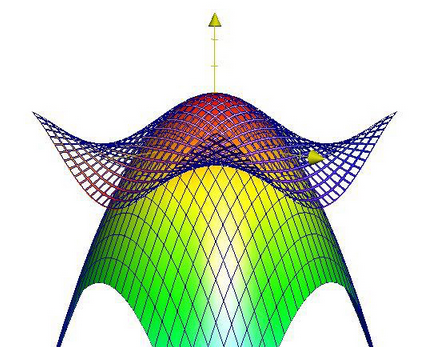
\includegraphics[width=0.3\textwidth]{figure_man/taylor_2D_quadratic.png}
    \caption*{\footnotesize $f$ and its second order approximation is shown by the dark and bright grid, respectively.
        (Source: \url{daniloroccatano.blog})}
\end{figure}

$\implies$ Hessians provide information about \textbf{local} geometry of a function.

\end{vbframe}
  
\endlecture

\end{document}
  
  